\section{Results}

Above all PIX is designed to produce efficient instrumented code. In order to test how efficient the
instrumented code actually is we ran experiments on a selection of benchmarks from the the SPEC CPU2000
Integer benchmark suite. All of the experiments described here, unless otherwise noted, were run on
one core of a quad-core 2.4GHz IA32 Intel Xeon running Red Hat linux Enterprise 4.1.2 (linux kernel 2.6.18).

The first set of experiments is intended to quantify the overhead of the program reorganization technique 
described in section \ref{Subsection:Relocation} to prepare the code for instrumentation to count
the basic block executions in the code. Recall that this technique adds an extra unconditional
branch to each function call in order to relocate the function, extends all of the branches in the code
to use 32-bit offsets, and pads each basic block whose size is fewer than 5 bytes with nops so that a
5 byte jump can be inserted. We perform these transformations on our benchmark set then run the resulting executable
to see the performance effects of our function relocation method has on the unaltered executable. Figure \ref{Figure:RelocOverhead} presents
the runtime overhead seen in the modified executable as a percentage of the original application runtime.
This figure shows that the maximum slowdown of these modifications is 6.5\%, with an
average slowdown of just 1.6\%. Of the popular dynamic instrumentation toolkits we have discussed so far (Pin, 
DynamoRIO, Valgrind and Dyninst), the smallest amount of overhead for performing no instrumentation with a dynamic instrumentation toolkit
on the x86 platform is when using DynamoRIO, which introduces an average of 38\% overhead and a maximum of 113\% overhead on the benchmark
set we present here \cite{luk2005pin}. This shows that the relocation method that in use by PIX has a minimal
performance impact on the performance of the application and thus is a suitable approach for use as a basis for
producing efficient instrumented code.

\begin{figure}[ht]
\centering
\label{Figure:RelocOverhead}
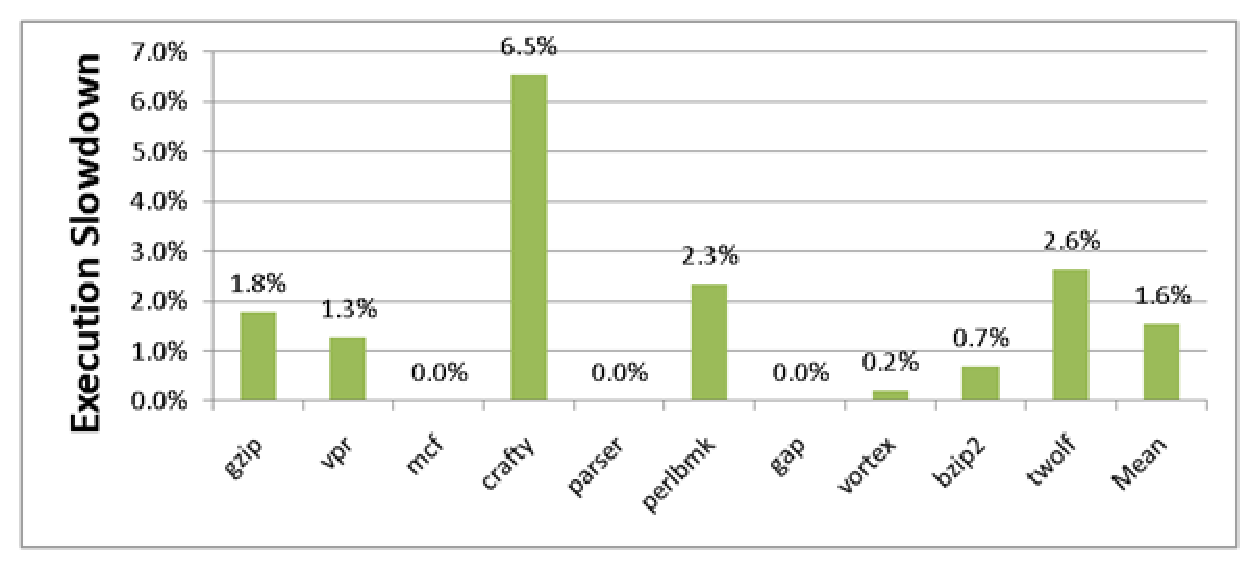
\includegraphics[scale=0.6]{relocperf.eps}
\caption{Application slowdown caused by preparing the code for instrumentation but without
any instrumentation inserted.}
\end{figure}

The next set of experiments shows how much overhead is necessary to perform the full task of counting the
basic block executions in the code. We use this particular instrumentation tool because basic block counting
is a typical example of an instrumentation tool where we would expect PIX to outperform other leading
dynamic instrumentation toolkits. Much of the work performed in basic block counting (updating a single
counter every time a basic block is encountered) can be done easily using a fast instrumentation snippet rather than
by a full instrumentation function. These counters embodied in the instrumentation snippets must also be
persistent throughout the entire run of the application, which is more suited to a static instrumentation approach
because the static instrumentation does not utilize any resources to determine whether instrumentation can be removed.
The basic block counting instrumentation tool is used to produce an instrumented
executable for each program in our benchmark suite, whose runtime is compared to the runtime of the 
unmodified executable. The results of this experiment are shown in figure \ref{Figure:ToolOverheads} as
how much overhead is introduced as a percentage of the original application runtime. The
resulting overhead of our basic block counter is an average of 84\%, compared to average overheads of
135\% for Pin, 396\% for DynamoRIO, 660\% for Valgrind, and 5701\% for Dyninst. This represents a savings of
51\% of the original application runtime when using PIX over the next most efficient option, Pin. Furthermore,
Pin uses a variety of optimizations such as tracking eflags bit liveness \cite{luk2005pin} that are currently
unincorporated into PIX. Our future plans (see Section \ref{Section:Future}) for this project include the addition of several
such optimizations already in use by Pin, which should only further improve on the efficiency of the instrumented
code produced by our tool.

\begin{figure}[ht]
\centering
\label{Figure:ToolOverheads}
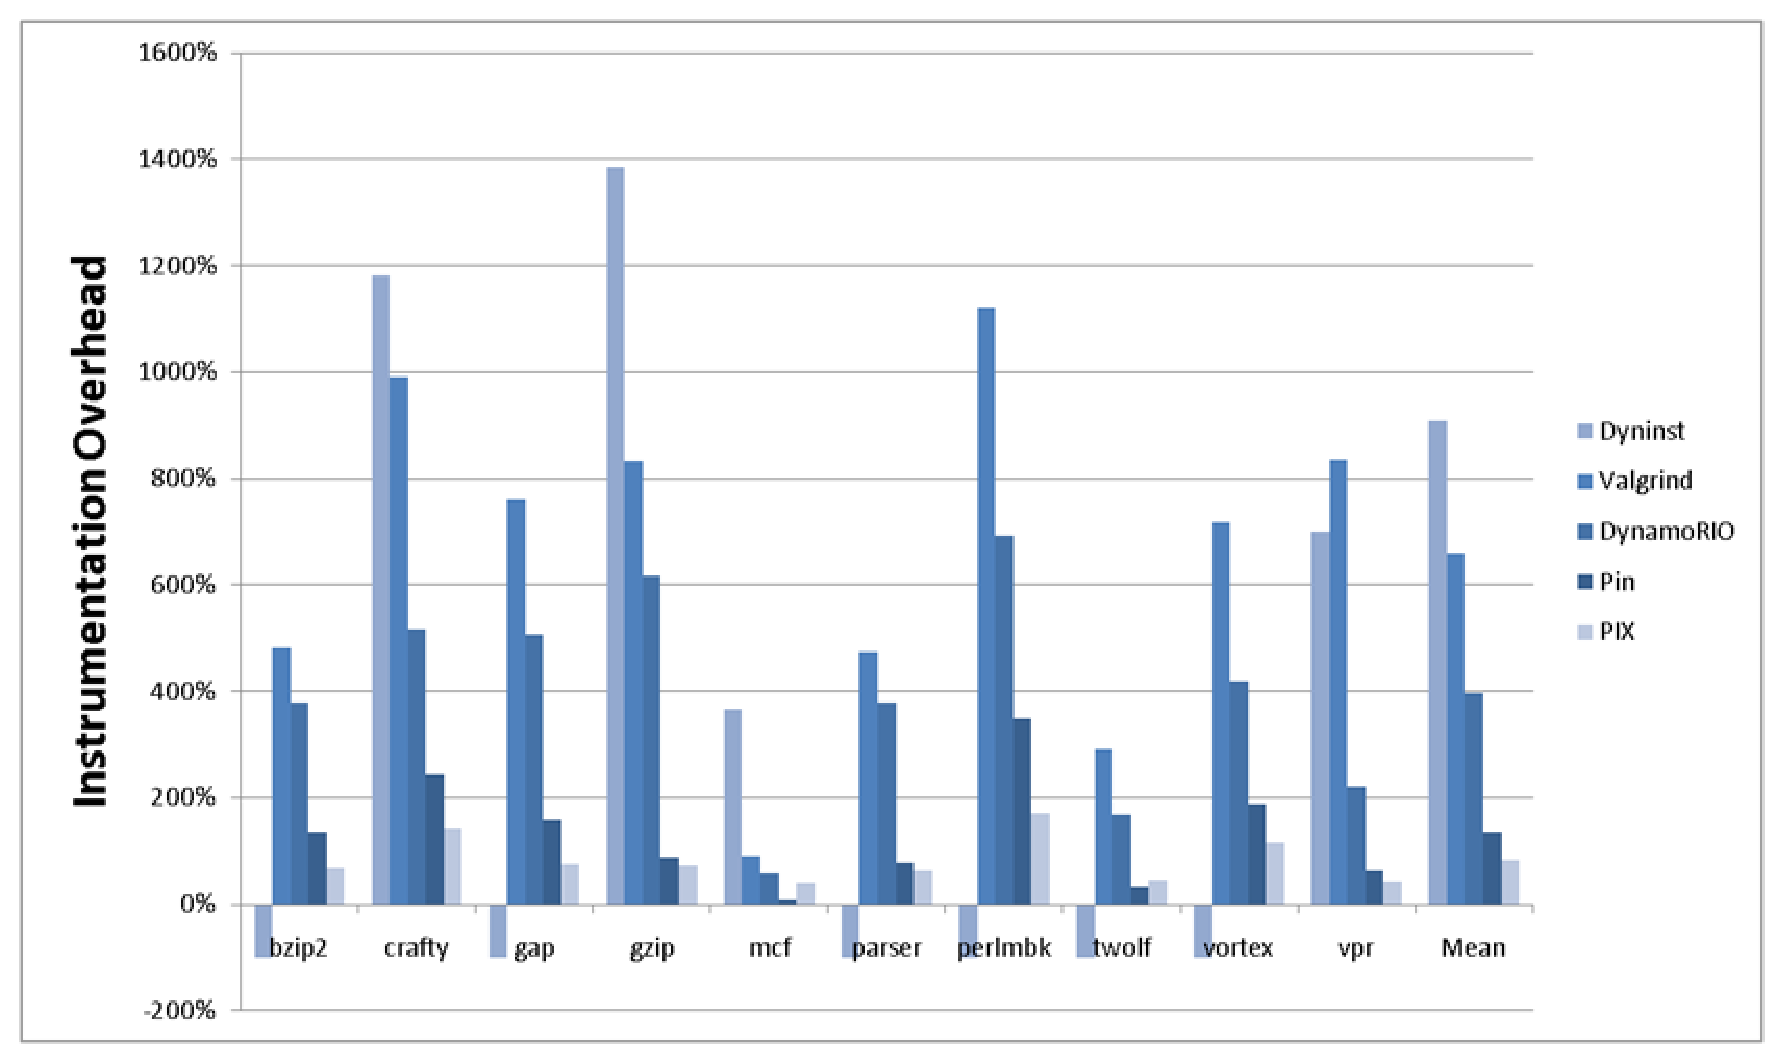
\includegraphics[scale=0.5]{bbcount.eps}
\caption{Performance of several x86 instrumentation tools with basic block counting instrumentation.}
\end{figure}